\documentclass[twoside]{article}
\input{ISC18-english.sty}
%%%%%%%%%%%%%%%%%%%%%%%%%%%%  Make sure to compile twice for proper cross-references. %%%%%%%%%%%%%%%%%%%%%%%
%%%%%%% For proper display of references, compile the document twice. %%%%%%%%%%%%%%%%%%%%% 
%%%%%%%%%%%%%%% If using TeX Live, compile using pdflatex command %%%%%%%%%%%%%%%%%%%%%%%
\begin{document}
\thispagestyle{empty}
%%%%%%%%%%%%%%%%% Article title header  %%%%%%%%%%%%%%%%%%%%
\fancyhead[LE]{Adaptive hybrid Active-Passive Learning}
%%%%%%%%%%%%%%%%% Article authors header   %%%%%%%%%%%%%%%%%%%%
\fancyhead[RO]{Moradi and Kasani}
\begin{center}
{
\includegraphics [height=25mm, width=150.3mm] {Images/isc18E}} \\
\vspace*{-1.8cm}
%\begin{center}
%\color{blue} 
%{\hspace{0.1cm}\rule{\textwidth}{1mm}}\\
%\end{center}
\vspace*{4cm}
%%%%%%%%%%%%%%%%% Article title  %%%%%%%%%%%%%%%%%%%%
{\Large \bf An Adaptive Hybrid Active-Passive Learning Strategy for Statistical Representativeness: A Case Study of Breast Cancer Diagnosis}\\
%%%%%%%%%%%%%%%%% Article authors and affiliations %%%%%%%%%%%%%%%%%%%%
{\bf
Mohammad Moradi\footnote[1]{{\bf Mohammad Moradi:} {\tt moradi\_m@razi.ac.ir }}, Elnaz Kasani$^2$  \\
$^1$Associate Professor, Department of Statistics, Razi University \\
$^2$Ph.D. Candidate in Statistics, Razi University}
\end{center}
\rule{\textwidth}{0.2mm}\\
%%%%%%%%%%%%%%%%% Article abstract  %%%%%%%%%%%%%%%%%%%%
\noindent{\bf Active learning reduces the cost of supervised learning by selecting informative observations for labeling, yet the resulting samples often lack statistical representativeness, leading to biased estimates of population parameters such as disease prevalence. In this study, we propose an adaptive hybrid strategy that initially employs margin-based sampling to rapidly improve predictive accuracy and then switches to simple random sampling once a predefined accuracy threshold is reached, thereby preserving the representativeness of the labeled sample. The proposed method is evaluated on the Wisconsin Breast Cancer dataset using a Random Forest classifier. Monte Carlo experimental results demonstrate that the hybrid strategy achieves predictive performance comparable to that of pure active learning while substantially improving the statistical representativeness of the labeled sample, thus providing a reliable foundation for valid statistical inference alongside high classification accuracy.}\\


\noindent{\bf Keywords:} 
Active learning,
Hybrid learning,
Random Forest,
Statistical inference,
Breast cancer diagnosis.  \\
\noindent{\bf Mathematics Subject Classification (2020):} $\rm 62H30$, $\rm 62D05$, $\rm 68T05$. \\
\hspace{1cm}\rule{\textwidth}{0.2mm}\\
%%%%%%%%%%%%%%
\section{Introduction}
 Obtaining labeled data is often substantially more expensive than collecting unlabeled observations. Active learning (AL) addresses this challenge by selecting only a subset of informative observations for labeling, thereby reducing annotation costs while maintaining high predictive performance. Over the past two decades, active learning has been successfully applied to numerous domains, including medical diagnosis, image analysis, natural language processing, and remote sensing \cite{Settles2009}, \cite{Lewis1994}, and \cite{Tong2001}.

Among the various active learning strategies, uncertainty-based methods are the most widely used. These methods select observations for which the current classifier is least confident, assuming that labeling such observations provides the greatest improvement in the decision boundary. Popular uncertainty criteria include least-confidence, entropy, and margin sampling. \cite{Settles2009}, \cite{Seung1992}.

Although existing active learning algorithms are highly effective from a predictive perspective, they are primarily designed to maximize classification accuracy, sensitivity, specificity, or the area under the ROC curve (AUC). Consequently, relatively little attention has been paid to the statistical properties of the selected sample. Since uncertainty sampling deliberately favors observations located near the classification boundary, the labeled sample generally does not constitute a representative subset of the underlying population. As a result, statistical quantities estimated directly from the labeled data, such as class prevalence or disease proportion, may be biased. Existing active learning algorithms optimize prediction but generally ignore statistical representativeness. This paper proposes a hybrid strategy that explicitly addresses both objectives.

This issue is particularly important in biomedical applications. For example, in breast cancer diagnosis, the primary objective is to classify tumors as benign or malignant accurately. However, clinicians and public health researchers are also interested in estimating the prevalence of malignant tumors in the target population. Such estimation requires representative samples, a property naturally provided by probability sampling but generally absent in conventional active learning.

Another characteristic of uncertainty-based active learning is the diminishing improvement in predictive performance during later iterations. The learning curve usually increases rapidly at the beginning because highly informative observations are selected first. As more observations are labeled, however, the curve gradually approaches a plateau, indicating that additional uncertainty-based selections contribute only marginal improvements to prediction accuracy. Continuing deterministic uncertainty sampling beyond this stage therefore provides little predictive benefit while further reducing the representativeness of the sample.

Motivated by this observation, we propose an adaptive active learning strategy that combines uncertainty sampling with random sampling. During the initial stage, observations are selected according to the margin uncertainty criterion, allowing the classifier to improve rapidly by labeling the most informative instances. Active learning continues until the predictive accuracy reaches a predetermined threshold, indicating that the classifier has attained the desired level of performance. From that point onward, the remaining observations are selected for labeling using simple random sampling. This adaptive strategy preserves the high predictive accuracy achieved during the active learning phase while improving the representativeness of the labeled sample, thereby providing a more reliable basis for subsequent statistical inference.


The proposed approach is evaluated using the Wisconsin Breast Cancer Diagnostic dataset with Random Forest classifiers. In addition to conventional classification accuracy, we evaluate the representativeness of the labeled sample by comparing the estimated proportion of malignant cases with the true population proportion. Experimental results demonstrate that the proposed hybrid sampling strategy achieves predictive performance comparable to conventional active learning while substantially improving the inferential quality of the labeled sample.

The main contributions of this paper are summarized as follows:

\begin{itemize}
\item We propose an adaptive hybrid active--passive learning strategy that combines uncertainty sampling with simple random sampling through an accuracy-based switching mechanism.

\item The proposed method preserves the rapid improvement in predictive performance achieved by active learning while improving the statistical representativeness of the labeled sample.

\item Unlike conventional active learning studies that focus solely on predictive performance, the proposed framework explicitly evaluates the inferential quality of the selected sample by assessing the accuracy of estimating the population proportion.

\item Experimental results based on the Wisconsin Breast Cancer dataset demonstrate that the proposed hybrid strategy achieves classification performance comparable to conventional active learning while substantially reducing estimation bias and improving the reliability of statistical inference.
\end{itemize}

\section{Active Learning Based on Margin Sampling}
Pool-based active learning assumes that a large pool of unlabeled observations is available, while obtaining class labels is expensive. The objective is to sequentially select a subset of observations whose labels are expected to maximize the improvement of the classification model. Among the various query strategies, margin sampling is one of the most widely adopted uncertainty-based methods because of its simplicity and effectiveness \cite{Settles2009}, \cite{Tong2001}.

Suppose the training pool consists of a labeled set
$
 L=\{(x_i,y_i),\,i=1,\ldots,n_L\}, 
$
and an unlabeled set
$
U=\{x_j,\,j=1,\ldots,n_U\}, 
$
where $n_L + n_U = N$. Initially, a small number of observations are selected randomly and labeled to construct the initial classifier. At each iteration, the classifier is trained using the current labeled set $L$, and posterior class probabilities are estimated for every observation in the unlabeled pool $U$.

For a classification problem with $k$ classes, let
$
P(y=k\mid x)
$
denote the posterior probability that observation $x$ belongs to class $k$. After sorting these probabilities in decreasing order,
\begin{equation*}
P_{(1)}(x)\ge P_{(2)}(x)\ge\cdots\ge P_{(K)}(x),
\end{equation*}
the margin score is defined as
\begin{equation*}
m(x)= P_{(1)}(x)- P_{(2)}(x). 
\end{equation*}
A small margin indicates that the classifier is almost equally uncertain between the two most probable classes, implying that the observation lies close to the current decision boundary. Consequently, observations with the smallest margin are considered the most informative for improving the classifier.

At iteration $t$, the next batch of observations is therefore selected according to
\begin{equation*}
B_t= \operatorname*{arg\,min}_{\mathbf{x}\in U} m(\mathbf{x}), 
\end{equation*}
where $B_t$ contains the $b$ observations having the smallest margin values. Their true labels are obtained from an oracle (e.g., a medical expert), after which they are transferred from the unlabeled pool to the labeled training set. The classifier is then retrained using the enlarged labeled dataset, and the procedure is repeated until a predetermined labeling budget is exhausted.

\begin{algorithm}[ht]
\caption{Adaptive Hybrid Active--Passive Learning}
\label{alg:hybrid}
\begin{algorithmic}[1]
\Require Unlabeled pool $U$, initial labeled size $n_0$, labeling budget $n_1$, batch size $b$, accuracy threshold $A_0$
\Ensure Trained classifier and labeled sample $L$

\State Randomly select $n_0$ observations from $U$ and obtain their labels.
\State Move the selected observations to the labeled set $L$.
\State Train the Random Forest classifier using $L$.

\While{$|L|<n_1$}

    \State Evaluate the classifier on the validation (or test) set and compute the classification accuracy $A$.

    \If{$A<A_0$}
        \State Compute the margin score for every unlabeled observation,
        \[
        m(x)=P_{(1)}(x)-P_{(2)}(x)
        \]
            \State Select the $b$ observations having the smallest margin values.
    \Else
        \State Select $b$ observations uniformly at random from the remaining unlabeled pool.
    \EndIf

    \State Reveal the true labels of the selected observations.
    \State Update the labeled set $L$ and unlabeled pool $U$.
    \State Retrain the Random Forest classifier.

\EndWhile

\State \Return Final classifier and labeled dataset.
\end{algorithmic}
\end{algorithm}
Algorithm~\ref{alg:hybrid} summarizes the proposed adaptive
hybrid strategy. The algorithm begins with uncertainty-based
sampling and automatically switches to simple random sampling
once the predictive accuracy reaches the predefined threshold
$A_0$.
\section{Experimental Dataset}

The proposed methodology was evaluated using the Wisconsin Breast Cancer
Database distributed in the \texttt{mlbench} package in R
\cite{Mangasarian1990,Street1993}. The dataset contains 699 patient records
described by nine cytological attributes measured on an ordinal scale from 1 to
10. After removing observations with missing values, 683 records remained,
including 444 benign and 239 malignant cases.

%In each experiment, the data were randomly divided into training and testing
%sets using stratified sampling (80\%--20\%). The training set was considered as
%the unlabeled pool. An initial labeled sample of size 10 was selected randomly,
%and observations were subsequently labeled according to the considered sampling
%strategy until a maximum budget of 300 labeled observations was reached.

\section{Simulation and Numerical Study}

To compare the predictive performance and statistical representativeness of the
three sampling strategies, two evaluation criteria were considered. The first
criterion was the classification accuracy evaluated on an independent test set.
The second criterion was the representativeness of the labeled sample, measured
by the absolute difference between the malignant proportion estimated from the
labeled sample and the corresponding population proportion. Lower values of this
measure indicate a more representative labeled sample. The following figures
summarize the average results over 50 independent repetitions.


In each repetition, the complete dataset was randomly divided into training and testing subsets using stratified sampling (80\%--20\%) to preserve the original class proportions. The training subset was regarded as the unlabeled pool, from which observations were sequentially selected for labeling. An initial labeled sample of size $n_0=10$ was selected at random from the training pool to train the first Random Forest classifier.

At each subsequent iteration, a new batch of observations, say $b=5$, was selected for labeling according to the sampling strategy under consideration. In the active learning approach, observations were selected using the specified uncertainty sampling criterion. In the passive learning approach, observations were selected by simple random sampling throughout the entire labeling process. In the proposed hybrid approach, observations were initially selected using the active learning criterion until the predictive accuracy reached a predetermined threshold, after which all remaining observations were selected by simple random sampling. The true labels of the selected observations were then revealed, the labeled training set was updated, and the classifier was retrained. This iterative procedure continued until the maximum labeling budget, ($n_1$), was exhausted.


After each iteration, the updated classifier was evaluated using the independent test dataset. Let $A_r(n)$
denote the classification accuracy obtained in the r-th repetition when the number of labeled observations equals $n$. Since each repetition produces a slightly different learning trajectory, the overall learning curve was obtained by averaging the classification accuracies over all repetitions,
\begin{equation*}
	\bar{A}(n) = \frac{1}{R} \sum_{r=1}^{R} A_r(n)
\end{equation*}
where R is the total number of repetitions. 

Besides predictive performance, the representativeness of the labeled sample was also investigated. Let $p$ 
denote the true proportion of malignant cases in the complete training population and let
$
	\hat{p}_r(n)
$
represent the corresponding proportion estimated from the labeled sample in the r-th repetition after $n$ observations have been labeled. For each repetition, the absolute estimation error was computed as
$
	D_r(n) = \left| \hat{p}_r(n) - p \right|
$
The representativeness curve was then obtained by averaging these absolute differences over all repetitions,
\begin{equation*}
	\bar{D}(n) = \frac{1}{R} \sum_{r=1}^{R} \left| \hat{p}_r(n) - p \right|
\end{equation*}

To quantify the variability among repetitions, the standard error of the mean absolute difference was calculated at each labeling stage, and approximate $95\%$ confidence bands were constructed as:
\begin{equation*}
	\bar{D}(n) \pm 1.96 \, SE(\bar{D}(n))
\end{equation*}
Figures 1--3 compare the active, passive, and proposed hybrid
learning strategies with respect to predictive accuracy and
sample representativeness.

\begin{figure}[ht]
\begin{center}

\includegraphics[width=7cm,height=6cm]{Images/Fig2.eps}

\includegraphics[width=7cm,height=6cm]{Images/Fig1.eps}\\
\vspace{-0.2cm}
\caption{\footnotesize{
Performance of conventional margin-based active learning. Accuracy improves
rapidly but the representativeness of the labeled sample deteriorates as more
uncertainty-based observations are selected.
}}\label{fig1}
\end{center}
\end{figure}


\begin{figure}[ht]
\begin{center}
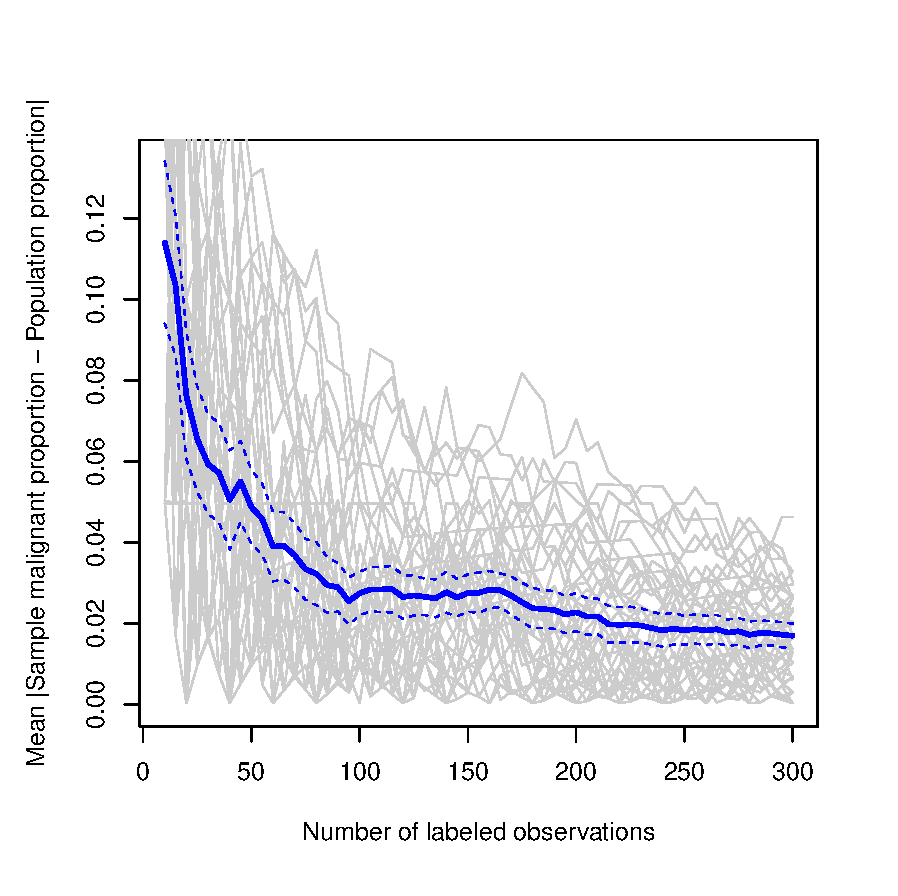
\includegraphics[width=7cm,height=6cm]{Images/Fig4.eps}
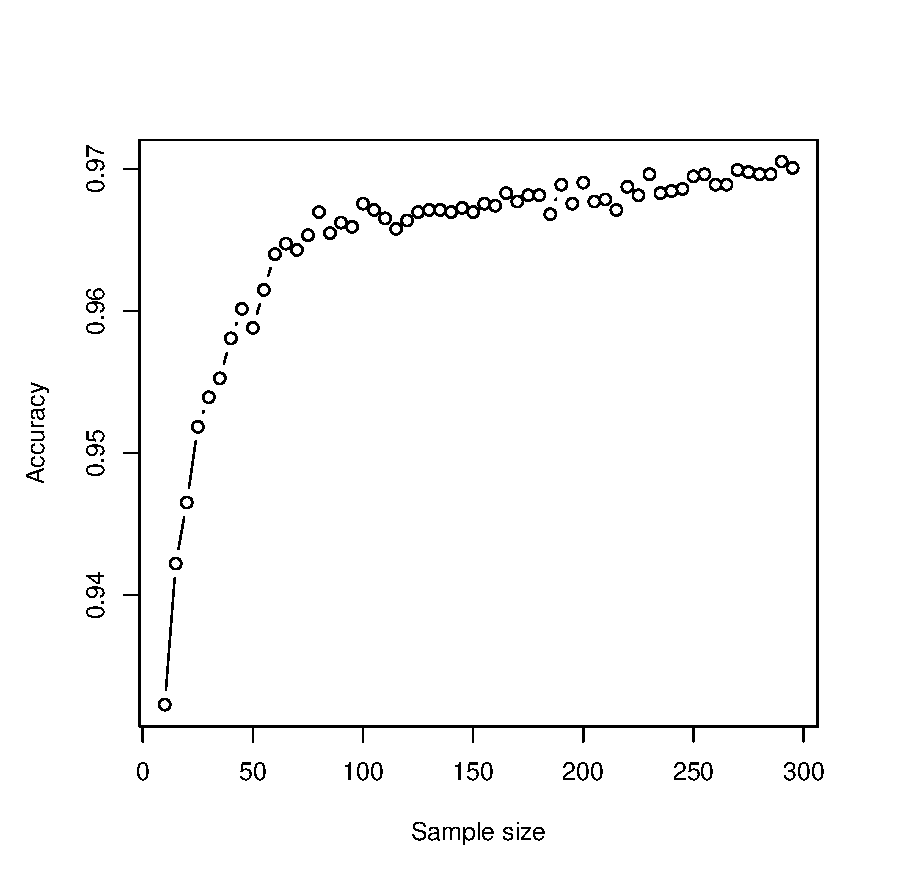
\includegraphics[width=7cm,height=6cm]{Images/Fig3.eps}\\
\vspace{-0.2cm}
\caption{\footnotesize{
Performance of passive learning using simple random sampling. Accuracy improves
gradually while the labeled sample becomes increasingly representative of the
population.
}}
\label{fig2}
\end{center}
\end{figure}


\begin{figure}[ht]
\begin{center}
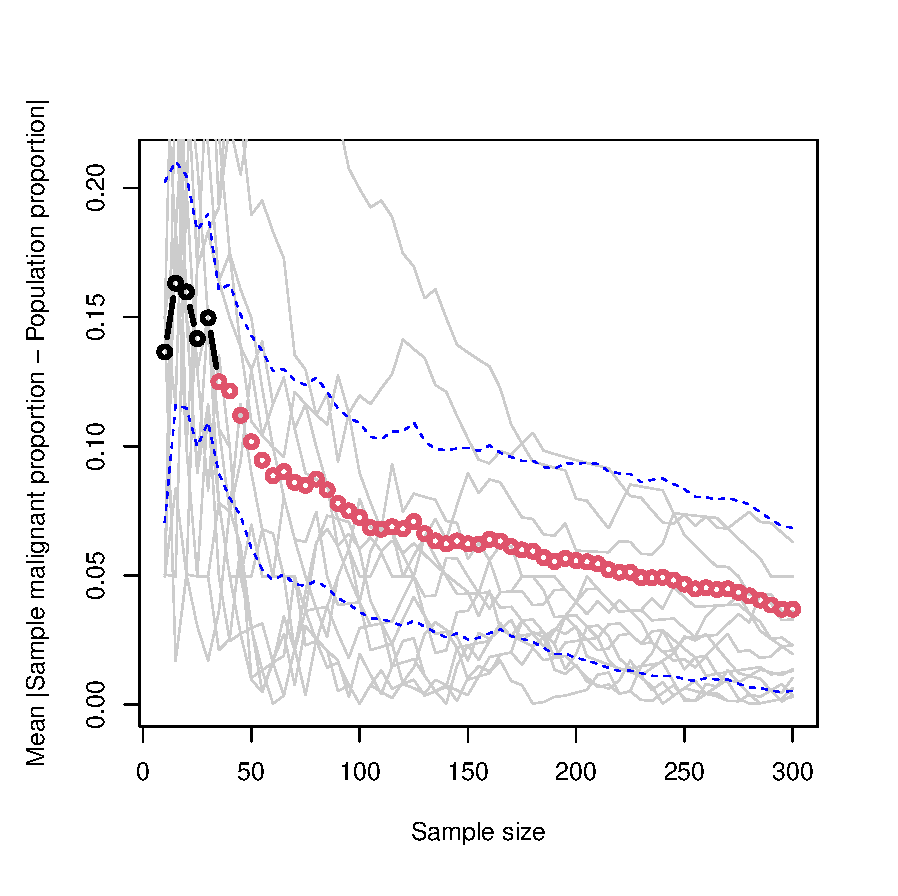
\includegraphics[width=7cm,height=6cm]{Images/Fig6.eps}
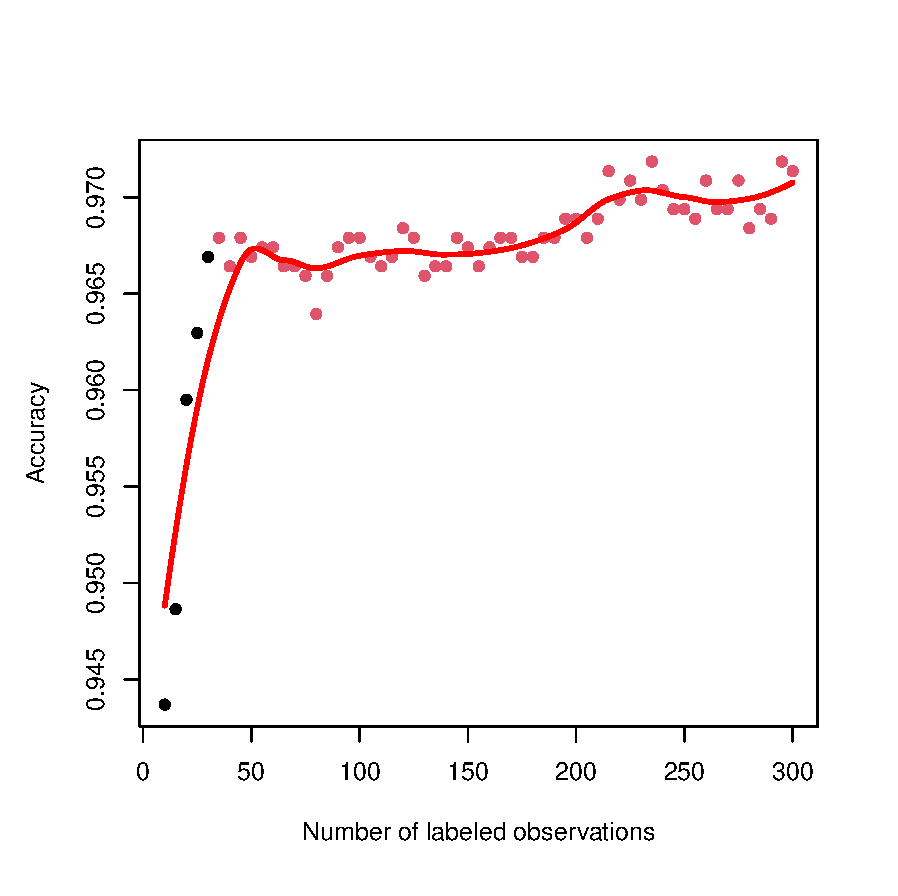
\includegraphics[width=7cm,height=6cm]{Images/Fig5.eps}\\
\vspace{-0.2cm}
\caption{\footnotesize{
Performance of the proposed hybrid active--passive learning strategy. Active
learning rapidly reaches the accuracy threshold, after which random sampling
improves sample representativeness while maintaining predictive performance.
}}\label{fig3}
\end{center}
\end{figure}

%%%%%%%%%%%%%%

\section*{Discussion and Conclusion}   
Conventional margin-based active learning improves classification accuracy but
reduces sample representativeness. The proposed hybrid strategy addresses this
trade-off by switching to random sampling after reaching a predefined accuracy
threshold, thereby maintaining predictive performance while enabling reliable
statistical inference.


%%%%%%%%%%%%%%%%%%%%%%%% References %%%%%%%%%%%%%%%%%%%%%%%%%%%%%
\newpage
\begin{thebibliography}{9}
		\bibitem[Lewis and Gale (1994)]{Lewis1994}
	Lewis D.D. and Gale W.A. (1994), A Sequential Algorithm for Training Text Classifiers, {\it Proceedings of SIGIR}.
		\bibitem[Mangasarian and Wolberg (1990)]{Mangasarian1990}
	Mangasarian O.L. and Wolberg W.H. (1990), Cancer diagnosis via linear programming, {\it SIAM News}, 23(5), 1--18.
	\bibitem[Settles (2009)]{Settles2009}
	Settles B. (2009), Active Learning Literature Survey, {\it Computer Sciences Technical Report 1648}, University of Wisconsin--Madison.
	\bibitem[Street et al. (1993)]{Street1993}
	Street W.N., Wolberg W.H., and Mangasarian O.L. (1993), Nuclear feature extraction for breast tumor diagnosis, {\it IS\&T/SPIE International Symposium on Electronic Imaging}.
	\bibitem[Seung et al. (1992)]{Seung1992}
	Seung H.S., Opper M. and Sompolinsky H. (1992), Query by committee, {\it Proceedings of the Fifth Annual Workshop on Computational Learning Theory (COLT)}, 287--294.
		\bibitem[Tong and Koller (2001)]{Tong2001}
	Tong S. and Koller D. (2001), Support Vector Machine Active Learning with Applications to Text Classification, {\it Journal of Machine Learning Research}.
\end{thebibliography}
 \end{document}

